\section{Results}
Each of the once-through transition scenarios are compared on multiple 
criteria: the number of advanced reactors deployed, the energy profile, 
the mass of enriched 
uranium required, the amount of \gls{SWU} capacity required to enrich uranium,
and the mass of waste produced. 

\subsection{Scenario 1}
Scenario 1 models only the \glspl{LWR} deploying the United States with no 
perscribed energy demand. As expected, the energy 
produced by the \glspl{LWR} follows with the number of reactors deployed
(Figure \ref{fig:energy1}). The maximum number of \glspl{LWR} deployed is 
, and reactors are deployed in 2025. 

\begin{figure}
    \centering
    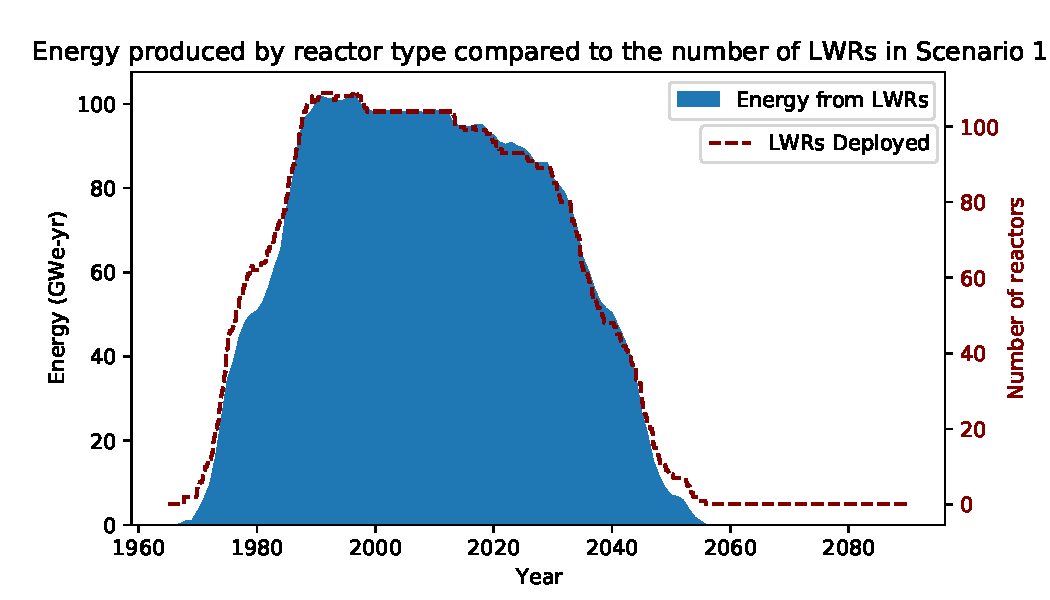
\includegraphics{energy_scenario1.pdf}
    \caption{Energy produced and the number of reactors deployed in Scenario 1.}
    \label{fig:energy1}
\end{figure}

\subsection{Reactor deployment}

\subsection{Uranium resources}

\subsection{SWU capacity}